\documentclass{emulateapj}
%\documentclass[manuscript]{aastex}

\usepackage{graphicx}
%\usepackage{subfigure}
\usepackage{verbatim}
\usepackage{natbib}
\usepackage{amsmath}
\bibliographystyle{apj}

\input blazar_environment_macros.tex

\shorttitle{BLAZAR ENVIRONMENTS AND CLUSTERING PROPERTIES}
\shortauthors{WILLETT ET AL.}

\begin{document}

\title{Environmental And Clustering Properties Of BL Lac and FSRQ Blazars}

\author{Kyle W. Willett et al.}
\affil{School of Physics and Astronomy, University of Minnesota, Minneapolis, MN 55455}

%%%%%%%%%%%%
%%% ABSTRACT
%%%%%%%%%%%%

\begin{abstract}
We present results from a large-scale study of the megaparsec:scale environments of blazars, including BL~Lac objects and flat-spectrum radio quasars. Using the catalog of galaxies from the Sloan Digital Sky Survey DR10 catalog, we compute spatial covariance amplitudes for a sample of 757~blazars. The covariance amplitudes are analyzed to compute the relative levels of clustering for various blazar types. We also compare the clustering of blazars to \FRI{} and \FRII{} radio galaxies to explore possibility of a parent population in the context of a blazar sequence. Finally, we present preliminary results on the morphologies of galaxies located within 1~Mpc of blazars, with classifications supplied by Galaxy Zoo data.
\end{abstract}

\keywords{blazars}

\section{Introduction} \label{sec:intro}

%%%%%%%%%%%%
%%% INTRODUCTION
%%%%%%%%%%%%

The standard model of blazars presumes that they are active galaxies with a jet closely aligned to the observer's line of sight. Observationally, blazars can be distinguished from other active galaxies with a variety of diagnostics, including extreme luminosities and non-thermal spectra dominated by relativistic beaming. 

The population of blazars displays significant observational diversity, however. The primary historical method of classification has been through the optical spectrum of the blazar, dividing them into two groups: BL~Lacs, characterized by weak or non-existent optical emission lines, and flat-spectrum radio quasars (FSRQs), which have strong, broad emission lines in their optical spectrum. An enduring question for many years has been whether BL~Lacs and FSRQs comprise physically distinct populations of galaxies, or whether a sequence exists between the two groups. 

Since highly-beamed emission from the relativistic jet often dominates the light observed from the blazar, studies of the object itself are challenging. As an alternative approach, we study the clustering properties of blazars in an attempt to determine their parent populations. Clustering studies benefit from the fact that they are assumed to be independent of the blazar's orientation to our line-of-sight. Differences in the clustering properties on scales of hundreds of kpc are already known to exist, for example, in the density-morphology relation \citep{dre80} and in the populations of powerful radio galaxies \citep{pre88}. 

Previous clustering studies of blazars have been limited by sample sizes of only a few tens. \citet{wur97} carried out a deep, largely subarcsec imaging survey of BL~Lac objects conducted at the CFHT. \citet{wur93} described the results pertaining to the host galaxies of 50 BL~Lac objects at $z<0.65$; \citet{wur97} report on the clustering environment of 45 of these 50 BL~Lacs. The remaining five objects either have unknown or very uncertain redshifts or we were unable to obtain deep, photometrically calibrated images of them, which prohibited successful clustering analysis.  

With this substantially larger (45 vs. 5) sample, \citet{wur97} confirmed the early result of \citet{pre88} that BL~Lac objects largely avoid rich clusters at low redshift and have distributions in $B$ richness measurements much more consistent with those of \FRII{} radio galaxies than with \FRI{}'s.  The typical environment of a BL~Lac object is a sub-Abell richness class 0 cluster with a CFHT sample mean of $\langle$\bgb$\rangle=209$~Mpc$^{1.77}$. Further, these results apply to all types of BL~Lac objects regardless of selection method (e.g., radio or X-ray selection) or detailed property (e.g., high or low optical polarization percentage, presence/absence of emission lines etc.) because no BL~Lac subtype has statistically distinct \bgb{} values. The only exceptions to this statement are correlations between redshift and \bgb{} and between host galaxy luminosity and \bgb{}, and a possible anticorrelation between \bgb{} and radio core dominance. 

\citet{smi95} computed \bgb{} for 16 BL~Lac galaxies and six \FRI{} galaxies; their respective correlation amplitudes were statistically indistinguishable for the small sample sizes, consistent with an Abell richness class of 0. 

Mention blazar envelope/sequence work, and possibility of how environment studies play into the larger scientific goal. 

With the release of the Sloan Digital Sky Survey (SDSS), we have for the first time a large and deep catalog with nearly uniform photometry and coverage out to redshifts greater than 1. We combine the SDSS data with the latest identifications of blazars, for which counts are now in the thousands. The larger sample size allows for the first time robust classification of blazar clustering properties, which we compare to other data to explore the possible parent population(s).

%%%%%%%%%%%%
%%% METHODS
%%%%%%%%%%%%

\section{Measuring the clustering properties}\label{sec:methods}

There are a number of diagnostics used to quantify the local density of galactic environments, including two- and three-dimensional correlation functions, luminosity density fields, $N^{{\rm th}}$-nearest neighbors, and distance to the nearest cluster or group. We analyze blazars by measuring the spatial covariance amplitude $B$ \citep{lon79}. A significant advantage of this method is that it can be applied to projected neighbors without knowing the true three-dimensional distribution of neighboring galaxies, which would be required for density field or nearest neighbor techniques. Accurate redshifts are not available for most galaxies in the survey we use (SDSS), especially at redshifts $z>0.2$. The technique is well-established in the literature of active galaxy environments \citep[e.g.,][]{pre88,yee87,ell89,wur97} and so our results can be compared to other studies. Finally, the method has been shown to be robust independent of the magnitude limit of observations or the counting radius of neighbors. The major disadvantage of the method is that it is a statistical measurement, and so uncertainties on individial measurements are typically quite large. We mitigate this by computing $B$ for several hundred sources and analyzing the statistics of the group, rather than focusing on individual objects. 

The technique for computing $B$ is briefly described here. For any population of objects as viewed on the sky in the far-field limit, its angular distribution can be approximated by:

\begin{equation}
\label{eqn:angcov}
n[\theta]d\Omega = N_g (1 + w[\theta]) d\Omega,
\end{equation}

\noindent where $n[\theta]d\Omega$ is the number of galaxies in a ring of solid angle $d\Omega$ at angular distance $\theta$ from the center of the ring. $N_g$ is the number of background galaxies in the ring, and the factor of $(1+w[\theta])$ expresses the probability of finding additional galaxies over the background level. $w[\theta]=0$ would correspond to a uniform angular distribution of galaxies in the universe (no clumping). 

The standard assumption, confirmed with deep optical observations of field galaxies, is that the angular distribution of galaxies follows a power law such that:

\begin{equation}
\label{eqn:wtheta}
w[\theta] = A\theta^{1-\gamma},
\end{equation}

\noindent where $A$ is the angular covariance amplitude and $\gamma$ an index describing the slope of the power-law distribution. The amplitude of $A$ for a particular system, then, determines the degree of clustering with respect to other similarly-scaled structures in the universe. 

Since this derivation has been completely general so far, we note that subscripts are used with computing the covariance amplitudes to indicate the type of object measured. For instance, $A_{gg}$ represents the galaxy-galaxy correlation amplitude, while $A_{gB}$ is the galaxy-BL~Lac correlation amplitude. 

Without a distance dependence, $A$ can be computed for any point on the sky by simply integrating Equation~\ref{eqn:angcov} from 0 out to $\theta$. This gives:

\begin{equation}
\label{eqn:angint1}
\int^\theta_0 n[\theta^\prime]d\Omega = \int^\theta_0 N_g (1 + w[\theta^\prime]) d\Omega.
\end{equation}

\noindent The solid angle subtended by an angle of $2\theta$ is $\Omega=2\pi(1-cos[\theta])$; for $\theta\ll1$, this translates to a differential:

\begin{equation}
d\Omega \simeq 2\pi \theta d\theta.
\end{equation}

\noindent Integrating Equation~\ref{eqn:angint1} over the angle yields:

\begin{eqnarray}
\int^\theta_0 n[\theta^\prime] 2 \pi \theta d\theta & = & \int^\theta_0 N_g (1 + w[\theta^\prime]) 2 \pi \theta d\theta \\
2\pi \int^\theta_0 \theta^\prime n[\theta^\prime]d\theta & = & 2 \pi N_g \int^\theta_0 \theta^\prime (1 + A {\theta^\prime}^{1-\gamma}) d\theta \\
N_t \left(\frac{\theta^2}{2}\right) & = & N_g \left(\frac{\theta^2}{2} + \frac{A\theta^{3-\gamma}}{3-\gamma}\right),
\end{eqnarray}

\noindent where $N_t$ is the integrated total number of galaxies within the circle. Solving for $A$, this gives:

\begin{eqnarray}
A = \frac{N_t - N_g}{N_g} \left(\frac{3-\gamma}{2}\right) \theta^{\gamma-1}.
\end{eqnarray}

Therefore, the angular covariance amplitude can be calculated for any galaxy as a function of the total number of galaxies in the field ($N_t$), the assumed background counts from a control field ($N_g$), the power-law index $\gamma$, and the field size $\theta$. We assume a canonical value of $\gamma=1.77$. The size of the field is determined by the scales used to derive the power-law dependence of $w[\theta]$; typical values are $\theta\leq1.5^\circ$. 

For a three-dimensional distribution of galaxies around some point in space, its spatial distribution can be parameterized as:

\begin{equation}
n[r]dV = \rho_g (1 + \xi[r]) dV,
\end{equation}

\noindent where $n[r]dV$ is the number of galaxies in a spherical shell at distance $r$ from the center. $\rho_g$ is the spatial density of background galaxies in the shell, and the factor of $(1+\xi[r])$ expresses the probability of finding additional galaxies over the background level. 

If the de-projected angular distribution in Equation~\ref{eqn:wtheta} is a power-law, then the spatial distribution will also follow a power-law with an index of $-\gamma$ (due to the increase in dimensions):

\begin{equation}
\xi[r] = Br^{-\gamma}.
\end{equation}

\noindent Here, $B$ is the spatial covariance amplitude, with subscripts indicating the pairs of objects for which the correlation function is computed (similar to $A$). 

\citet{lon79} project the spatial covariance function into angular space to establish a relationship between $A$ and $B$: 

\begin{equation}
\label{eqn:atob}
B = \frac{A~N_{bg}[m]}{I_\gamma} \frac{D^{\gamma-3}}{\Psi[M(m,z)]}.
\end{equation}

Substituting for $A$, this gives the final form:

\begin{equation}
\label{eqn:bgb}
B = (N_t - N_{bg})\frac{(3-\gamma) D^{\gamma-3} \theta^{\gamma-1}}{2 A_\theta I_\gamma \Psi[M(m,z)]}
\end{equation}

\noindent Here, $m$ is the apparent magnitude completeness limit of the observation; depending on the redshift $z$, this is translated into an absolute magnitude limit $M(m,z)$. $D$ is the angular diameter distance\footnote{\citet{lon79} give this value as the co-moving distance. Later derivations use the luminosity distance \citep[eg,][]{yee87,ell91}; the most recent references replace it with the angular diameter distance \citep{yee99,muz07,zau07}. I have not found an explicit reference to the correction.} to the source. $\Psi[M]$ is the normalized integral luminosity function of galaxies in the field down to brightnesses of $M$. $n_{bg}[m]$ is the surface density of background galaxies brighter than $m$, and $I_\gamma$ is an integration constant dependent on the index of the power-law. For the assumed value of $\gamma$, $I_\gamma=3.87$.  

Since $B$ is impossible to measure directly without explicit data on the three-dimensional positions of all objects in the field (often not possible for fields of view with many faint objects), the standard technique is to measure $A$ from deep exposures and use Equation~\ref{eqn:atob} to determine $B$. Therefore, measuring $B$ for any particular field requires:

\begin{itemize}
    \item $\theta$ - angular size of the field
    \item $m$ - apparent magnitude limit of the observation
    \item $z$ - redshift of the target
    \item $N_t$ - total number of galaxies in the field
    \item $N_g$ - the expected background counts of galaxies down to $m$
    \item $\Psi[m,z]$ - luminosity function of galaxies down to $m$ at redshift $z$
\end{itemize}

The uncertainty in a value of $B$ can also be calculated as a function of the total number of background and galaxy counts:

\begin{equation}
\label{eqn:deltab}
\frac{\Delta B}{B} = \frac{\sqrt{(N_t - N_{bg}) + 1.3^2 N_{bg}}}{N_t - N_{bg}} = \frac{\sqrt{N_t + 0.69 N_{bg}}}{N_t - N_{bg}}.
\end{equation}

\noindent This error estimate is considered to be conservative, including both the Poissonian error in the net counts $(N_t - N_{bg})$ and dispersion in the background counts ($N_{bg}$). The factor of $1.3^2$ is included to account for the clustered, non-Poissonian distribution of the background counts \citep{yee99}. 

The integrated luminosity function $\Psi[M(m,z)]$ is assumed to be in the form of a Schechter function, which is a combination of a power law at fainter luminosities and an exponential at brighter luminosities. In magnitudes, the differential Schechter LF is:

\begin{eqnarray}
\label{eqn:schechter}
\phi[M] dM = 0.4 ({\rm ln} 10) \phi^*~(10^{0.4(M^* - M)(\alpha + 1)}) \times \nonumber \\
{\rm exp}[-10^{0.4(M^*-M)}],
\end{eqnarray}

\noindent where \phistar~is the scaling for a volume-limited sample, \mstar~is the characteristic magnitude of the LF ``knee'' and $\alpha$ is the slope of the power-law portion of the LF. In theory, this function can be fit with data to determine all three parameters in a given field. In practice, \citet{yee87} and collaborators treat all three variables somewhat differently. $\alpha$ is assumed to be either $-1.0$ or $-1.2$, based on fits to previous galaxy fields; the covariance amplitude is relatively insensitive to this, since the LF is not typically not integrated down to more than two magnitudes fainter than \mstar. \mstar~is taken from previous optical surveys \citep{kin85,seb86} that computed Schechter LFs for different cosmologies and a weighted mix of galaxy morphologies. The absolute magnitudes are translated into $r$-band using color models of galaxy morphologies, and then $K$-corrected depending on the redshift of the cluster. Values for \mstar~range from $M_R\sim-22$ to $-19$ mags. Finally, the scaling value \phistar~is determined by integrating the luminosity function over the volume of the field and then scaling it to the observed control field counts at each redshift epoch. 

The integrated luminosity function for computing the covariance amplitude is:

\begin{equation}
\label{eqn:schechter_int}
\Psi[M] = S_n \int_{-\infty}^{M} \phi[M^\prime] dM^\prime, 
\end{equation}

\noindent where $M$ is the absolute magnitude corresponding to the observational limit of the survey. Since background galaxy counts rise much faster than the LF at magnitudes fainter than \mstar, \citet{yee87} count galaxies only up to the \underline{brighter} of two limits: the completeness magnitude of the survey ($M=m_c$) or $M=M^* + 2.5$. Since any given field is not volume-limited, the scaling factor $S_n$ normalizes the luminosity function in agreement with background galaxy counts. 

If the luminosity function for each field is being computed from the data, then galaxies in the field must have their apparent magnitudes $K$-corrected to the observed waveband. For the binned redshift distribution in \citet{yee87}, a differential $K$-correction corrects all observed $r$-band galaxies in the bin to the average redshift of the group; the colors for each morphology are taken from \citet{seb86}. In addition, evolution of the LF as a function of lookback time will also affect the total number of counts in each field. The effects can be summed into the characteristic magnitude for each morphological type $i$ as a function of redshift:

\begin{equation}
\label{eqn:mstar_morph}
M_i^*[z] = M_i^*[0] + K_i[z] + E_i[z],
\end{equation}

\noindent where $M_i^*[z]$ is summed over morphology type into an integrated LF, and then integrated again over volume so that it can be directly compared to the observed galaxy counts. 

%%%%%%%%%%%%%%%%%%%%%%%%%%%%%%
% General properties of sample
%%%%%%%%%%%%%%%%%%%%%%%%%%%%%%

\section{Sample}\label{sec:sample}

The parent blazar sample was assembled from available compilations in the literature. The primary source for blazar identification comes from the multi-frequency catalog Roma-BZCAT \citep{mas09}. BZCAT compiles known blazars from numerous surveys, primarily in radio and X-ray wavelengths. Photometric information includes the radio flux density at 1.4~GHz and the X-ray flux between 0.1--2.4~keV, as well as its $R$-band magnitude as determined from SDSS. We supplemented Roma-BZCAT with SDSS optically-selected BL~Lac \citep{plo10} and FSRQ candidates \citep{che09a}, along with gamma-ray selected blazars from TeVCat \citep{hor08}. 

\begin{figure}
%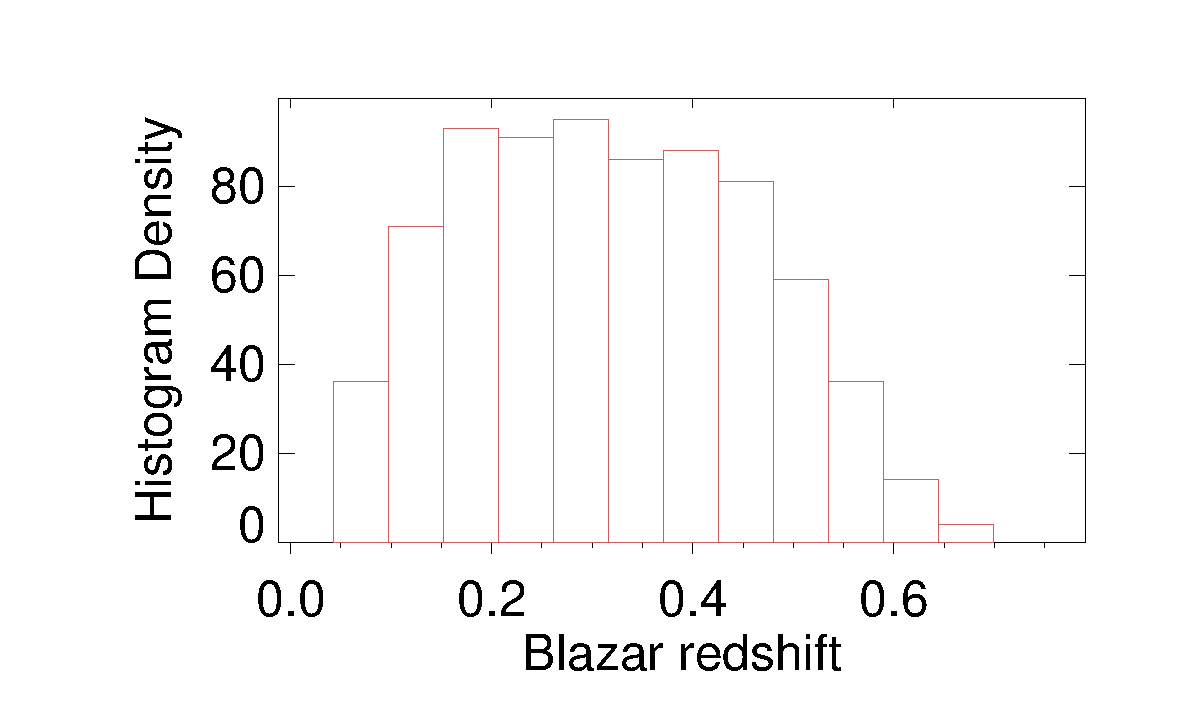
\includegraphics[width=3.5in]{blazar_zhist.eps}
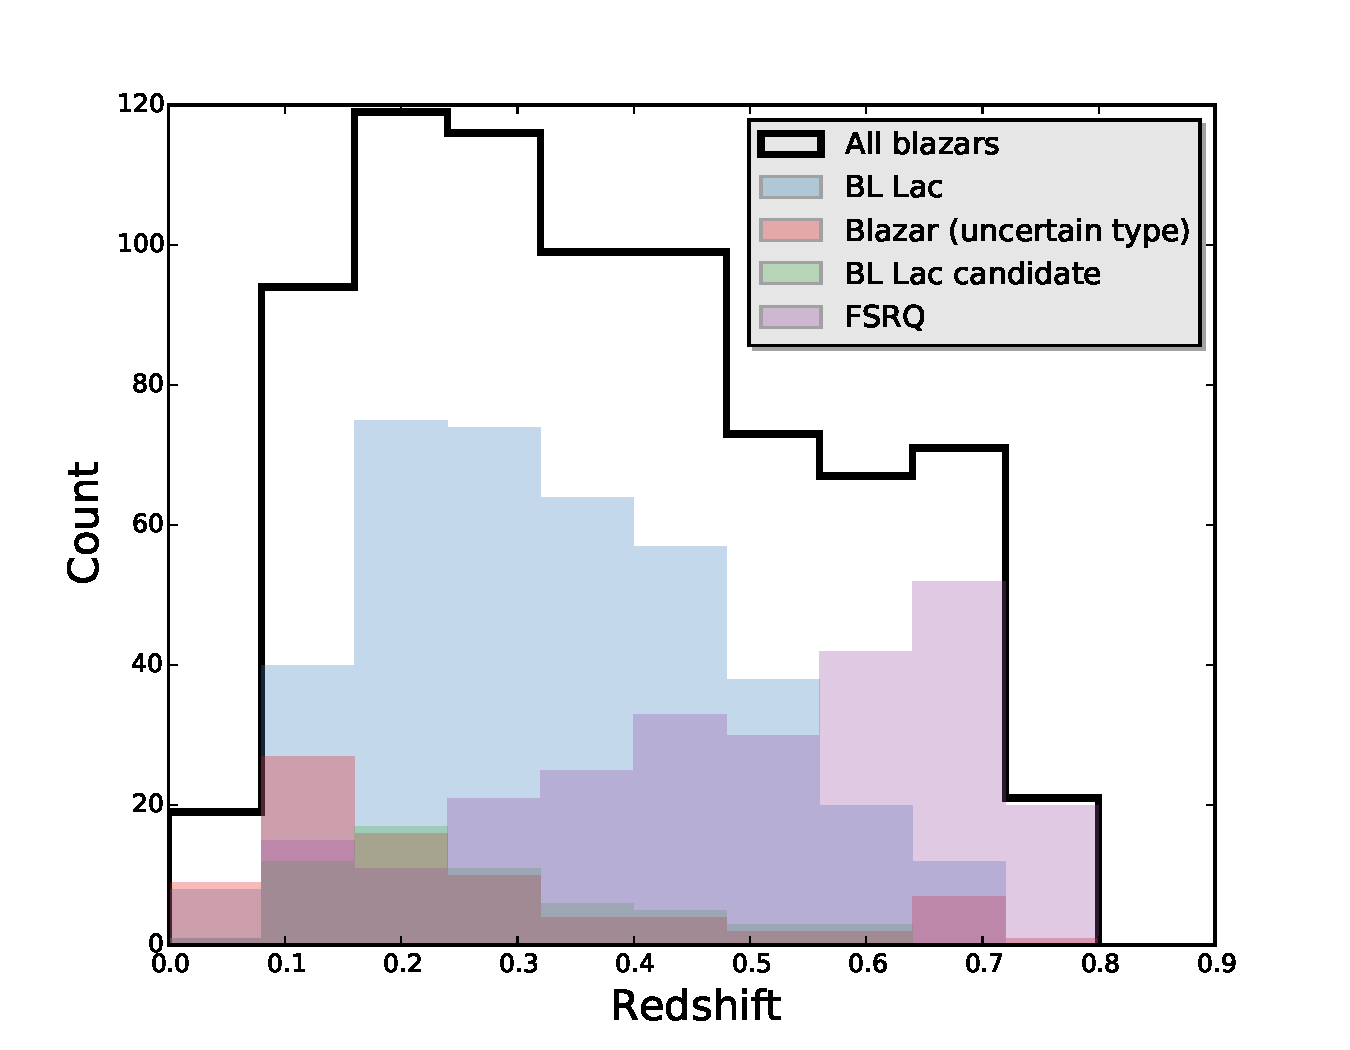
\includegraphics[width=3.5in]{figures/blazars_zhist.pdf}
\caption{Redshift distribution for the 778~blazars within the footprint of SDSS DR10 at $0.043<z<0.75$. BL~Lacs dominate the population at $z<0.5$, while FSRQs are more common at higher redshifts. 
\label{fig:blazar_zhist}}
\end{figure}

After removing duplicates, the combined catalogs yielded 2934~blazars. Figure~\ref{fig:blazar_zhist} shows their redshift distribution. The distribution varies significantly by blazar sub-type; FSRQs comprise 90\% of the blazars at $z>0.1$, with a mean redshift of $\langle z\rangle=1.34$. The BL~Lacs have a much lower average redshift, at $\langle z\rangle=0.37$. Unclassified blazars \citep[``QSO candidates'', as defined by][]{mas09} have a mean redshift of 0.30; however, a K-S test confirms that its redshift distribution is more consistent with BL~Lacs than QSOs. 

We then take the positions of each blazar and searched the SDSS DR10 catalog \citep{ahn13} for entries in the ``PhotoObj'' table for nearby neighbors, and restricting results to objects the SDSS pipeline identified as galaxies. The angular radius of the search for each blazar is set at a projected distance 500~kpc at the redshift of the blazar. The apparent magnitude down to which a galaxy is considered for counting is the brighter of: $M_r^* + 2 > M_{r,lim}$, where $M_{r,lim}$ is the absolute magnitude corresponding to the $r$-band completeness limit of the SDSS at the distance of the blazar. 

The value of \bgb{} is computed for each blazar using Equation~\ref{eqn:bgb}. Parameters for local galaxies ($z<0.15$) were taken from the SDSS~DR6 $r'$-band luminosity function of \citet{mon09a}, with $\phi^*=3.22\times10^{-3}$~Mpc$^{-3}$, $M_r^*=-21.47$, and $\alpha=-1.23$ (assuming $h=0.71$). For higher-redshift galaxies, we evolve the luminosity function in bins of $\Delta z=0.1$ out to $z=0.65$ using the $^{0.1}r$-band fits to all galaxies in the AGES survey \citep{coo12}. 

We confirm that computing the spatial covariance amplitudes for a uniformly random set of positions within the SDSS footprint yields an average $B$ value consistent with 0, verifying that our background subtraction is being correctly computed. 

Several additional constraints further lower the number of blazars on which clustering analysis can be performed. Although BZCAT is an all-sky catalog, only 1834 (63\%) of the objects fall within the SDSS footprint. Of those blazars, we analyze data only for blazars in the redshift range $0.043<z<0.75$. The lower limit is due to the practical consideration of searching large areas of sky within a projected radius of 500~kpc, which corresponds to an angular size of 10\arcmin. This eliminated 1.5\% of the blazars within the SDSS footprint. The upper redshift limit is set by the sensitivity of the SDSS; blazars at high redshifts will have fewer neighboring galaxies that can be detected with SDSS. For high redshift objects computing the \bgb{} coefficient will (statistically) include no neighbors that are physically associated with the blazar, and so the clustering coefficient approaches that of the background sky. The upper redshift limit is thus chosen so that our absolute counting magnitude corresponds to an $M^*$ galaxy at $z=0.75$, eliminating another 41\% of the blazars in the SDSS footprint. Finally, to ensure that measurements of \bgb{} are not dominated by low number counts, we analyze only blazars with at least 10 neighboring galaxies detected. The final sample contains 757~blazars, with 528~BL~Lacs, 98~FSRQs, and 131~unclassified blazars. 

%%%%%%%%%%%%
%%% RESULTS
%%%%%%%%%%%%

\section{Results}\label{sec:survey_results}

\begin{figure}
%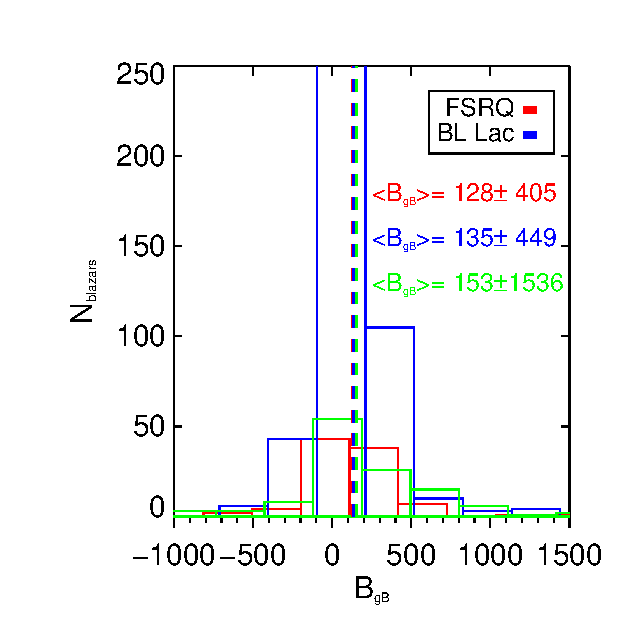
\includegraphics[width=3.5in]{bgb_hist.eps}
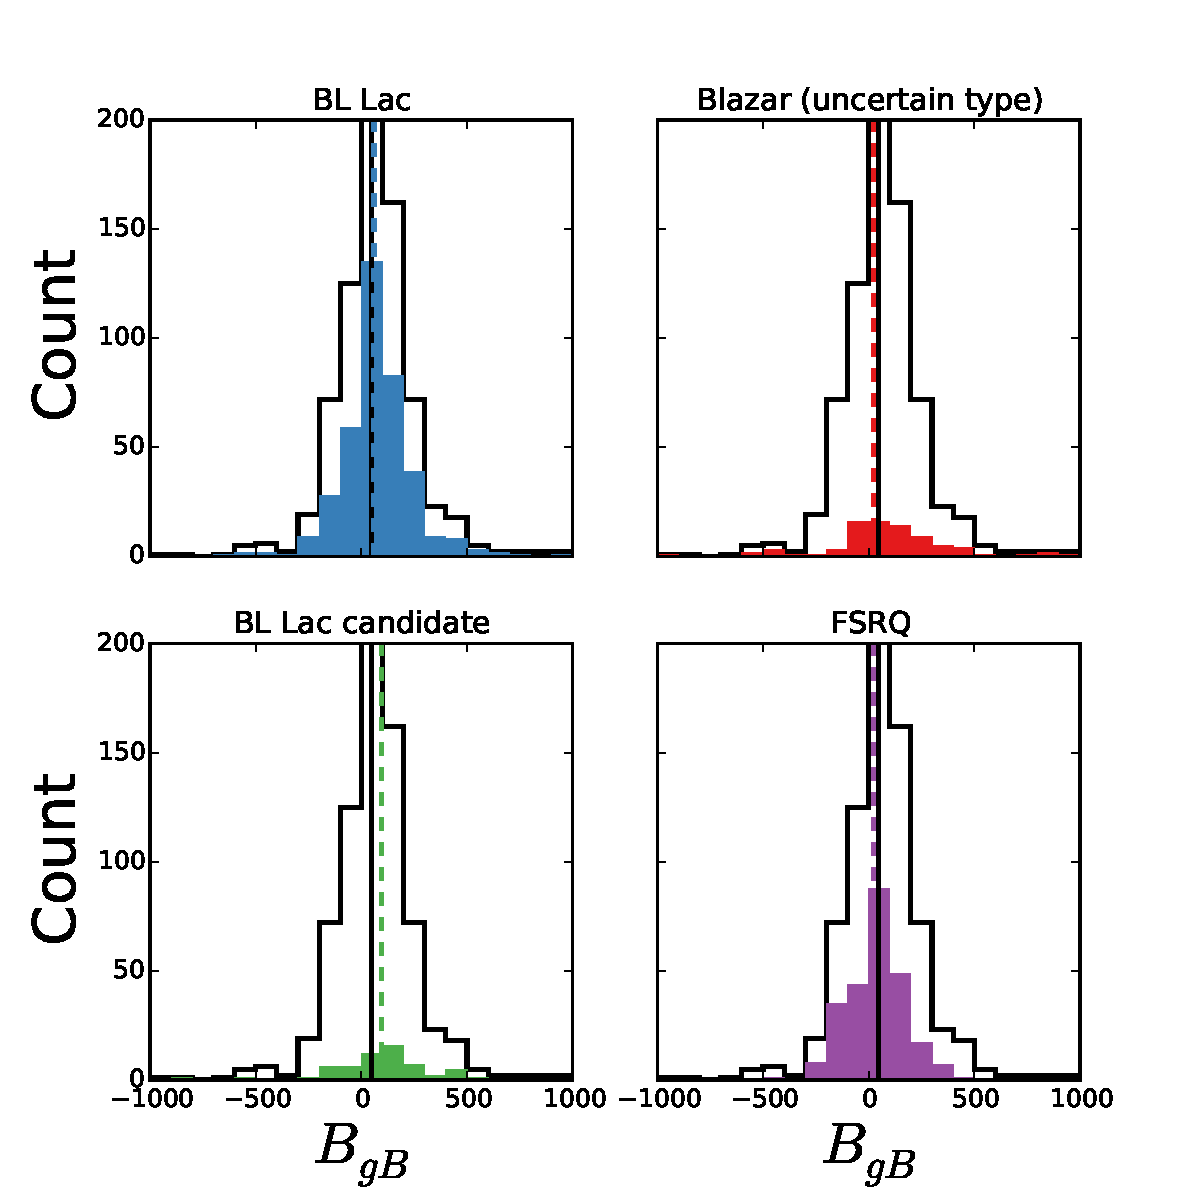
\includegraphics[width=3.5in]{figures/bgb_hist.pdf}
\caption{Distribution of spatial clustering amplitudes (\bgb) from SDSS imaging for various blazar sub-types. Dashed lines show the median \bgb{} values for both the overall blazar (solid) and sub-samples (dashed), respectively. All blazars have average \bgb{} values higher than the background; the average \bgb{} for BL Lacs and candidates is 2--3~times higher than that for FSRQs.
\label{fig:bgb_hist}}
\end{figure}

Figure~\ref{fig:bgb_hist} shows the distribution of the blazar clustering amplitudes (all spatial correlation amplitudes are reported in units of Mpc$^{1.77}$). The mean value for all blazars is $121$, confirming the basic conclusion that blazars tend to lie in moderately overdense regions of the universe. The spread of \bgb{} values for the blazars is large, ranging from $-2652$ to $5801$. Negative values of \bgb{} indicate that some blazars do lie in apparent voids; however, 71\% have clustering amplitudes greater than zero. According to the Abell richness class calibration of \citet{yee99}, this places xx\% of blazars in clusters with Abell classes of 0.

Splitting the sample by blazar type, the clustering amplitudes for BL~Lacs and FSRQs are remarkably similar. BL~Lacs have a mean \bgb{} of $148\pm312$, while FSRQs have $144\pm268$. A Kolmogorov-Smirnov test confirms that the distributions are not inconsistent with being drawn from the same population at a probability of $0.274~(1.0\sigma)$. Therefore, there is no evidence based on the clustering statistics that BL~Lacs and FSRQs inhabit different environments at redshifts $z<0.75$. 

Among the objects studied are 131 objects whose blazar type is defined by BZCAT as ``uncertain''. Discuss possibility of matching these to BL~Lac/FSRQ, information available on selection method, and whether the environmental technique might be used as a diagnostic for blazar type. Probably due to optical lines?

Results from our study can be compared to earlier results; however, differences in the parameters used in Equation~\ref{eqn:bgb} will cause systematic differences. The most immediate are the parameters used for the galaxy luminosity function $\Psi[M]$ and the cosmology used to compute the distance. For example, applying the cosmology assumed by \citet{wur97} ($q_0=0.02, \Omega_\Lambda=0, H_0=50~\mbox{km s}^{-1}\mbox{Mpc}^{-1}$) to our blazar sample raises the mean \bgb{} value from $121\pm436$ to $167\pm558$. Their luminosity function parameters are very similar to our own, with a slightly shallower slope ($\alpha=-1.0$), a $M_r^*$ value of $-20.9$, and a luminosity function evolution where $M$ evolves as $E(z)\sim z$. Adjusting only for the cosmology, our mean value for the BL~Lacs of $161\pm367$ is close to the \citet{wur97} value of $209\pm386$. 

The blazar \bgb{} values are relatively flat as a function of redshift for $z<0.5$. Between $z=0.5$ and 0.75, however, there is a significant increase in the average \bgb, increasing by a factor of $\sim2-3$. The same effect is seen for both BL~Lacs and FSRQs (Figure~\ref{fig:bgb_redshift}). Similar results were found for BL~Lacs by \citet{wur97}, who found that the median \bgb{} increased by a factor of four at $z>0.35$, and for which the trend is the same for both radio- and X-ray-selected BL~Lacs. Our results, which have $\sim10$ times as many objects, suggest that richer clusters begin to occur at a higher redshift; the medians of the samples when split at $z=0.35$ are almost identical. 

\begin{figure}
%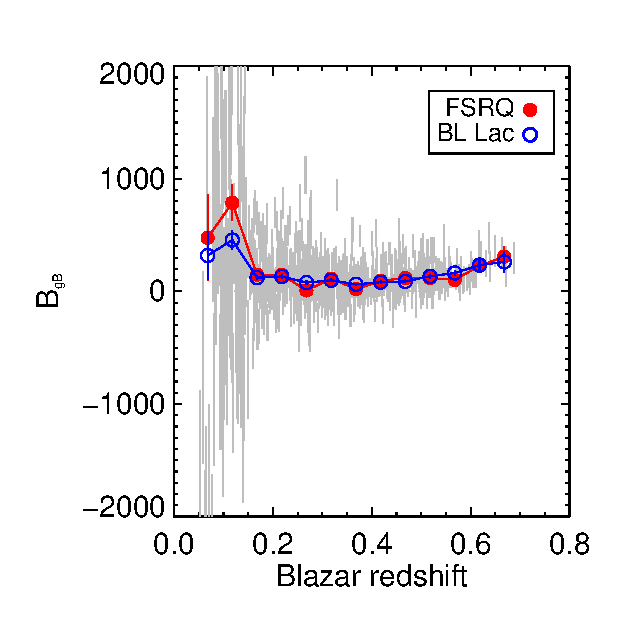
\includegraphics[width=3.5in]{bgb_redshift.eps}
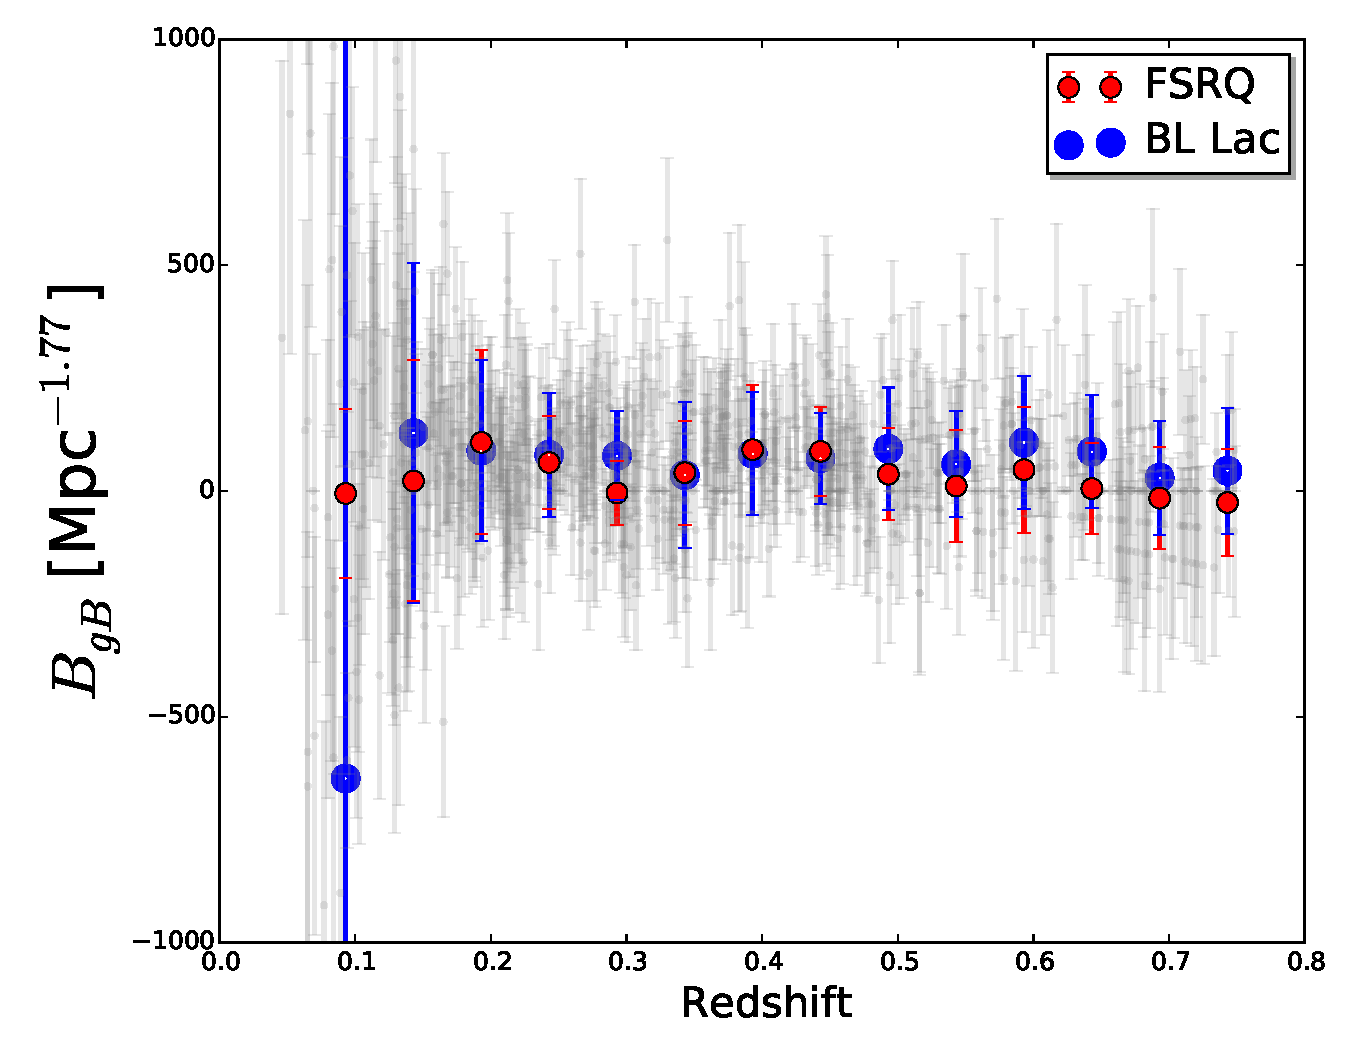
\includegraphics[width=3.5in]{figures/bgb_redshift.pdf}
\caption{\bgb{} for the blazars as a function of redshift. Grey points show measurements (with uncertainties) for individual blazars; blue and red circles show the binned mean values for \bgb{} for the BL~Lac and FSRQ sub-samples. 
\label{fig:bgb_redshift}}
\end{figure}

%%%%%%%%%%%%
%%% DISCUSSION
%%%%%%%%%%%%

\section{Discussion}\label{sec:survey_discussion}

\subsection{Comparison samples}\label{ssec:comparison}

Comparison samples:

\begin{itemize}
    \item CoNFIG \citep{gen08} - morphological classifications from NVSS-FIRST; spectroscopic redshifts for $\sim75\%$
    \item \citet{kim08} - radio galaxies from four surveys (NVSS + FIRST + WENSS + GB6); morphology is automated, restricted to ``simple'', ``compact'', and ``complex''
    \item morphological similarities; pure ellipticals and spirals from Galaxy Zoo
    \item random points on the sky 
\end{itemize}

We compare the clustering properties of blazars to active radio galaxies since, according to the unified model, these are the parent populations of blazars. As a result, the clustering properties of radio galaxies should be similar to those of blazars, assuming that the orientation of the jet has no effect on the megaparsec:scale environment. 

A concern for comparing clustering properties of other galaxy types to blazars is to avoid biases of sample selection wherever possible. One possible bias arises from the redshift distributions of any comparison sample. Results from Figure~\ref{fig:bgb_redshift} show a rise in $B$ values as a function of redshift. If we were comparing our blazars to galaxies with a higher average redshift, the clustering values would be similarly high. We therefore match the redshift distributions of any comparison sample using the following method: firstly, we consider only objects in the same redshift range ($0.043<z<0.75$) as for the blazars. Next, we bin the redshift distribution of the blazars with $\Delta z=0.02$ and count the number of objects per bin. We then truncate the comparison sample at the highest-redshift bin for which the number of blazars is greater than or equal to the number of comparison galaxies. For all bins at lower redshift, we randomly select comparison galaxies within that bin to search for neighbors and compute \bgb. 

The largest available catalogue of radio galaxies with robust morphological classifications is the \config~sample of \citet{gen08}. \config~consists of 274 bright radio sources at 1.4~GHz, with visually-classified \FRI{}/\FRII{} morphologies available for all galaxies. We searched the SDSS for neighbors of \config~galaxies with confirmed redshifts, which comprises 89\% of the total. We were able to compute $B$ values for 283 radio galaxies, of which 55 were \FRI{} and 184 were \FRII{}. The remaining 44 galaxies were classified by \citet{gen08} as compact sources, with no visibly extended radio lobes. 

For all radio galaxies in \config, the mean $B$ value is $164\pm389$, statistically similar to our blazar results. The subsamples of FR galaxies also have similar means, with \FRI{} galaxies at $150\pm533$ and \FRII{} galaxies at $175\pm364$. Compact sources showed a similar distribution of $B$ values, at $136\pm265$. A K-S test between the \FRI{} and \FRII{} galaxis showed no significant difference in their distribution. 

\citet{gen13} specifically measure the richness of radio galaxies using the richness method of \citet{win11}. They found that \FRI{} galaxies existed in richer environments than \FRII{} galaxies.

\citet[][KI08]{kim08} assembled a sample of radio sources with much larger numbers than \config, but without detailed, visually-classified morphologies. We used their sample of galaxies cross-identified in four radio surveys (FIRST, NVSS, WENSS, GB6) and one optical survey (SDSS; DR6) with spectroscopic redshifts. This yielded 2886~radio galaxies in the SDSS footprint, 1964 of which fell in the redshift range of the blazars. After matching a subsample of the radio galaxies to the blazar redshift distribution, we compute \bgb{} values for 258 galaxies between $0.063<z<0.627$.  

\bgb{} values for the \citet{kim08} galaxies were roughly a factor of two higher than the both the blazars and \config~radio galaxies, with a mean value of $299\pm342$. A higher percentage of these galaxies as compared to blazars also live in overdense regions, with 88\% of the KI08 sources having \bgb$<0$. 

Since there are too many galaxies in KI08 to be efficiently classified visually, the authors develop an automated morphological classification for the radio emission. This is based on two criteria: the difference in the amount of 1.4~GHz flux measured in two surveys (FIRST and NVSS) with different synthesized beam sizes, and the ratio of peak to integrated flux from the FIRST survey, which gives a dimensionless concentration index on a 5\arcsec~scale. Their classes of radio morphology are ``complex'', (simple) ``resolved'', and (simple) ``compact''. The comparison sample we selected contained 111~complex, 110~resolved, and 37~compact galaxies. 

Complex radio galaxies from KI08 inhabited the richest environments, with a mean \bgb{} value of $356\pm340$. In contrast, the clustering amplitudes for both radio galaxies with simple morphologies were similar, at $275\pm286$ for compact galaxies and $251\pm324$ for resolved galaxies. 

{\em Why is the clustering amplitude for KI08 twice that of \config?}

Finally, we looked at host galaxies using the GZ1 classifications to see how the morphology-density relation applies to blazar hosts, and whether the standard assumption that blazars are hosted in elliptical galaxies holds true. For optical galaxies, we used classifications from the Galaxy Zoo project \citep[GZ;][]{lin11}, using their clean classifications for ellipticals and spirals. As with the radio galaxies, we analyzed a sub-sample of the roughly 1 million galaxies with GZ classifications that matched the redshift distribution of the blazars. For elliptical galaxies, this allowed us to probe out to a redshift of $z=0.50$; spiral galaxies are much more limited, with a maximum redshift bin of $z=0.20$. 

The mean $B$ values for the galaxies selected by optical morphology are significantly different; elliptical galaxies resemble the blazar and radio galaxy distributions, with a mean covariance amplitude of $168\pm316$. Spiral galaxies have much lower $B$ values, however, with a larger spread and a mean close to zero ($12\pm359$). The K-S test applied to spiral galaxies and the blazar distribution (matching the spiral redshift range) is inconsistent at the 2.7$\sigma$ level. While the means for both are much closer, it should be noted that a K-S test is also inconsistent between the {\em elliptical} galaxy $B$ distribution and the blazars. This is more puzzling, since blazar hosts are thought to be almost without exception elliptical galaxies \citep{urr95}. 

\begin{deluxetable*}{lrccl}
\tabletypesize{\scriptsize}
\tablecaption{Measured spatial covariance amplitudes from SDSS imaging \label{tbl:bgtable}}
\tablewidth{0pt}
\tablehead{
\colhead{Galaxy sample} &
\colhead{$N$} &
\colhead{$\langle B_g \rangle$} &
\colhead{$\sigma_{Bg}$} &
\colhead{Reference}
\\
\colhead{} &
\colhead{} &
\colhead{[Mpc$^{1.77}]$} &
\colhead{[Mpc$^{1.77}]$} &
\colhead{}
}
\startdata
Blazars                                   & 757         & 121            & 436            & 1,2,3   \\
\hspace{10 pt} BL~Lac                     & 528         & 111            & 257            &         \\
\hspace{10 pt} FSRQ                       & 98          & 116            & 278            &         \\
\hspace{10 pt} Uncertain                  & 131         & 143            & 859            &         \\

Radio galaxies                            & 283         & 131            & 410            & 4       \\
\hspace{10 pt} FR I                       & 55          & 138            & 598            &         \\
\hspace{10 pt} FR II                      & 184         & 133            & 372            &         \\
\hspace{10 pt} Compact                    & 44          & 111            & 258            &         \\

Radio galaxies (optical counterparts)     & 258         & 269            & 357            & 5       \\
\hspace{10 pt} Complex                    & 111         & 321            & 357            &         \\
\hspace{10 pt} Compact                    & 37          & 282            & 434            &         \\
\hspace{10 pt} Resolved                   & 110         & 211            & 323            &         \\

Optical galaxies                          & 624         & 125            & 335            & 6       \\
\hspace{10 pt} Elliptical                 & 540         & 145            & 329            &         \\
\hspace{10 pt} Spiral                     & 84          & $-2$           & 348            &         \\

\enddata
\tablerefs{(1) - \citet{mas09}; (2) - \citet{plo10}; (3) - \citet{hor08}; (4) - \citet{gen08}; (5) - \citet{kim08}; (6) - \citet{lin11}}
\end{deluxetable*}

\subsection{The blazar sequence/envelope}\label{ssec:sequence}

\begin{figure}
%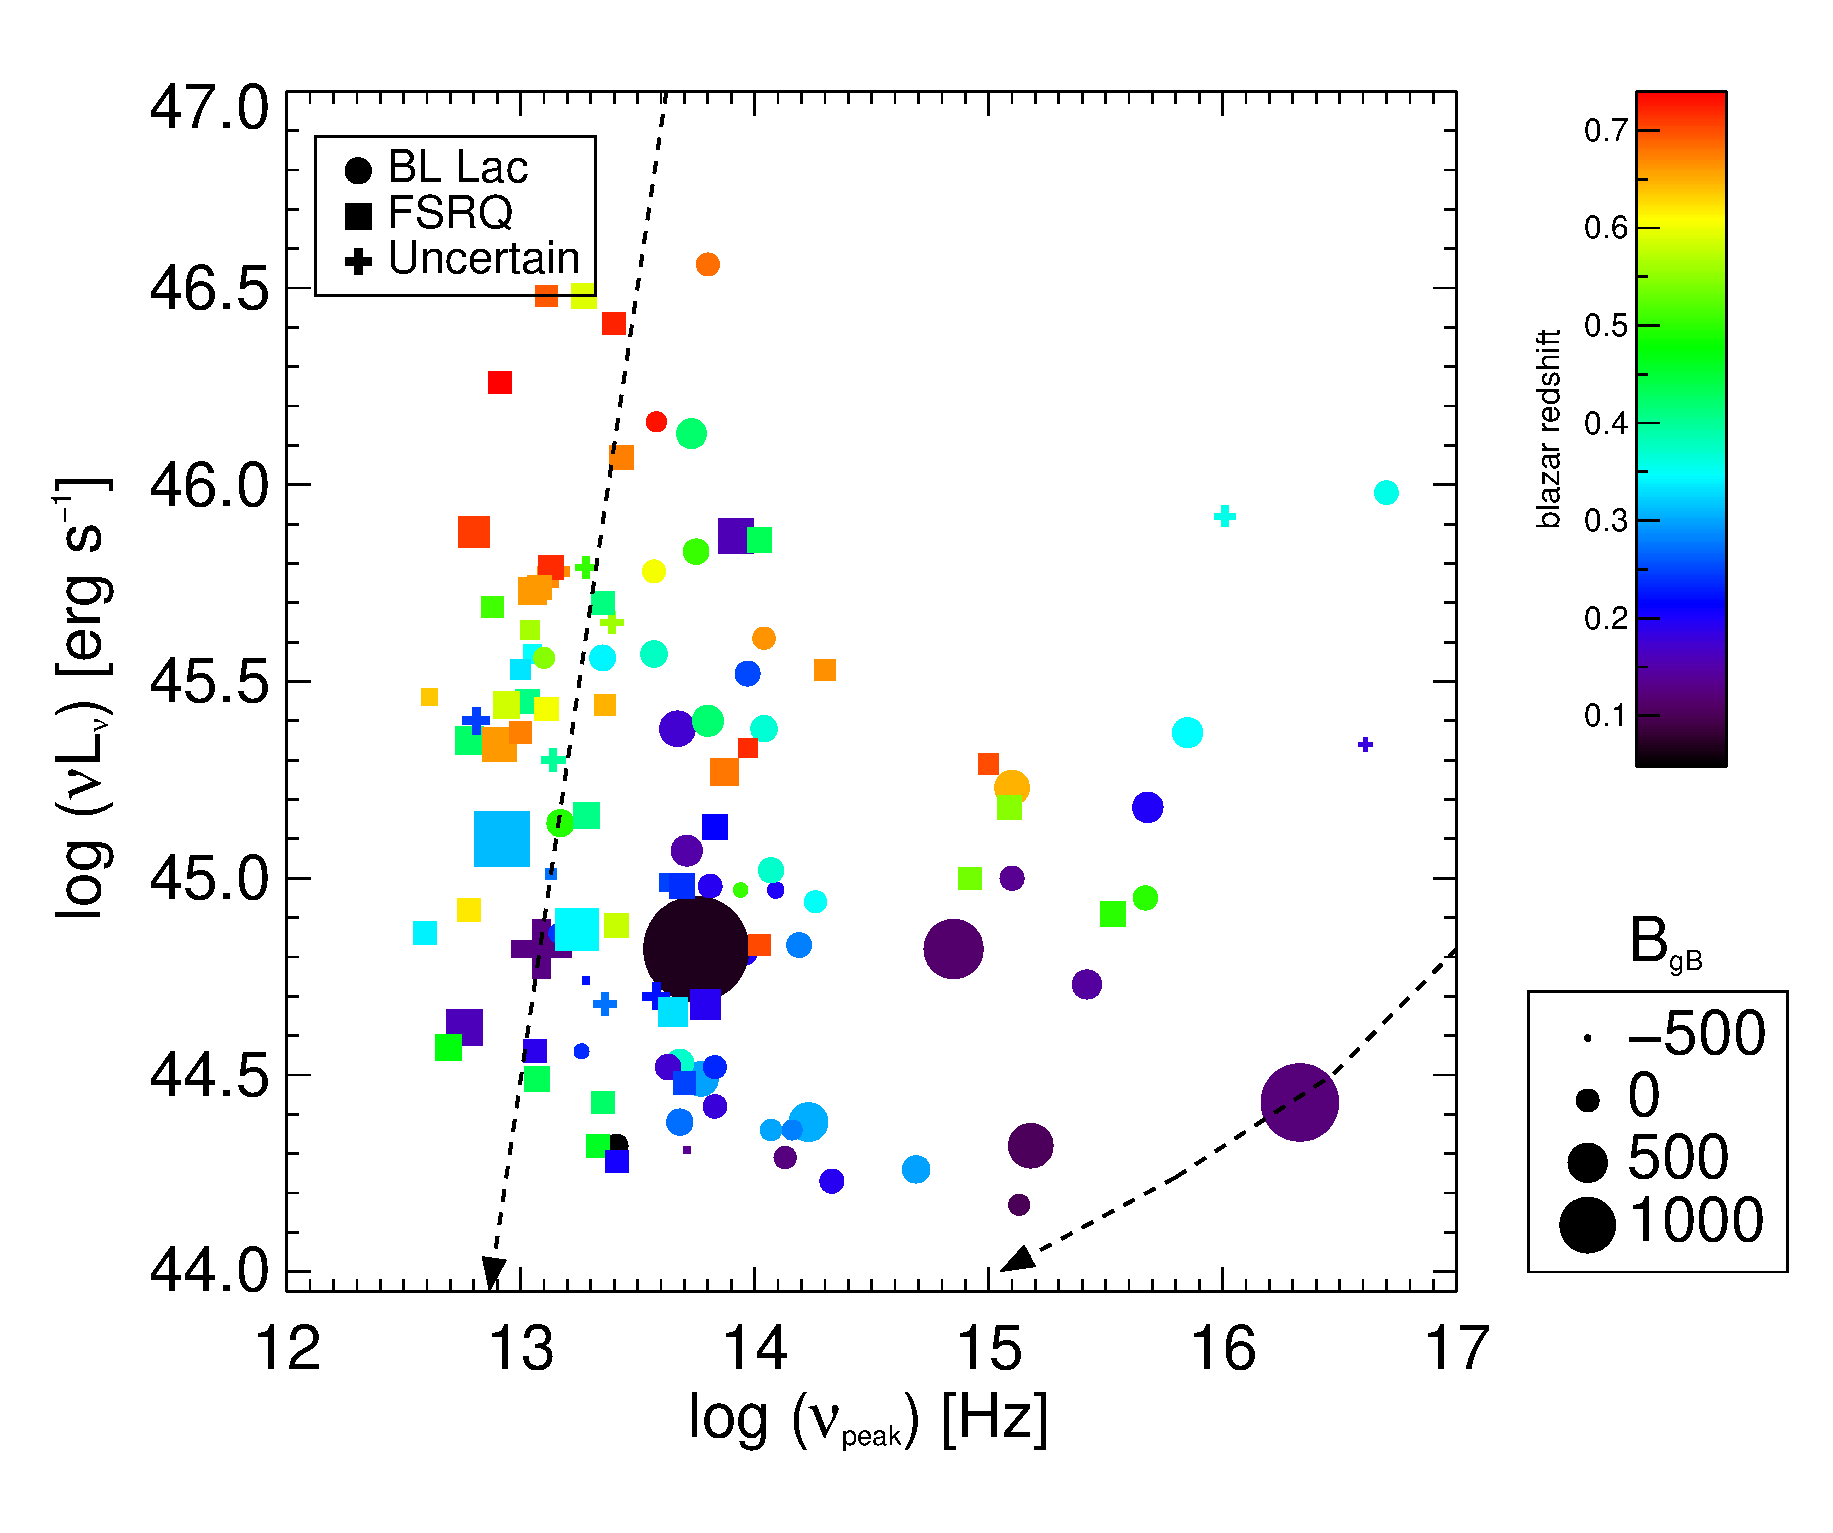
\includegraphics[width=3.5in]{bgb_blazarsequence_allseds.eps}
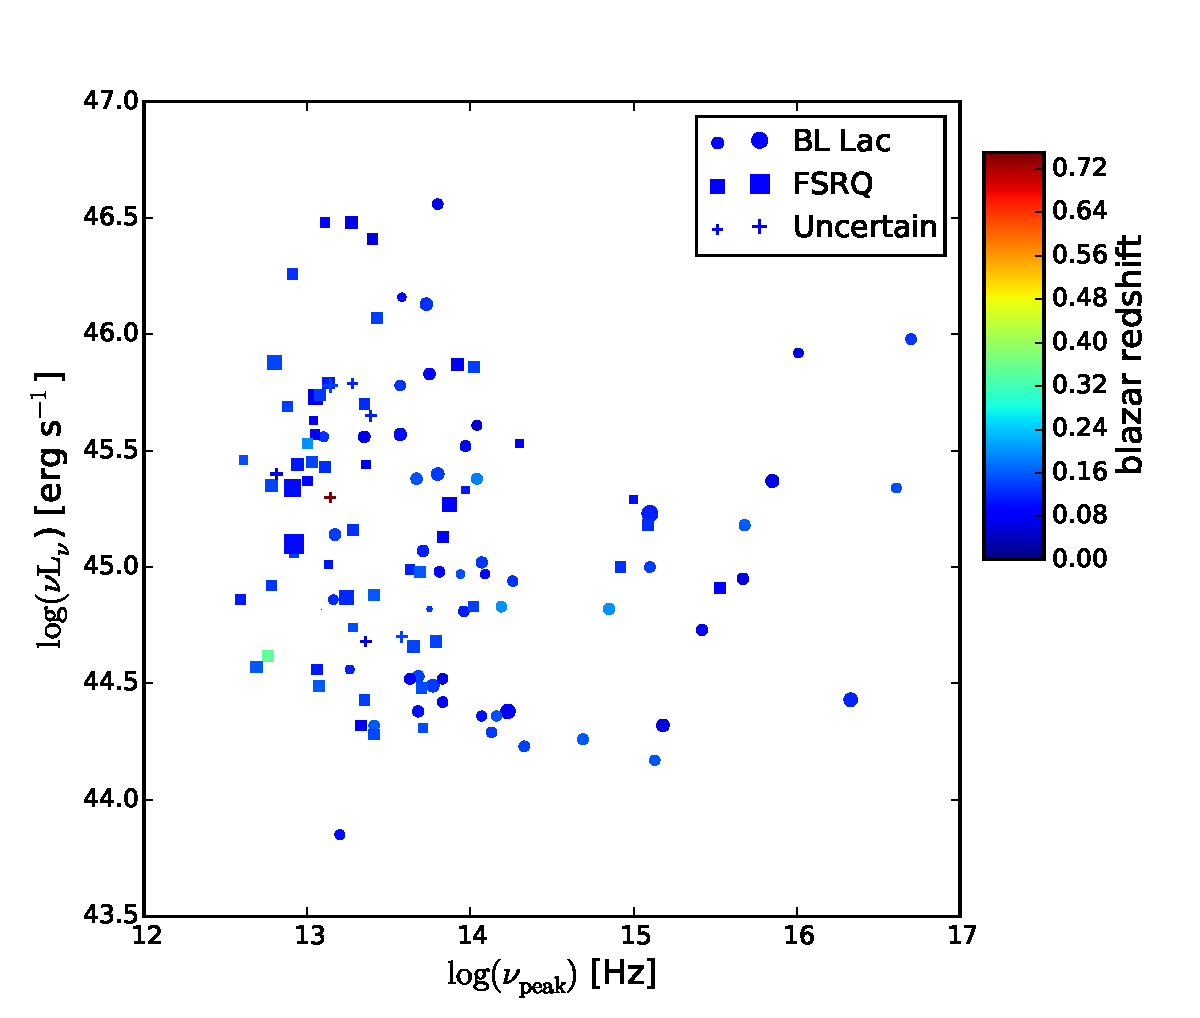
\includegraphics[width=3.5in]{figures/bgb_blazarsequence_allseds.pdf}
\caption{{\bf NOT YET PYTHON GENERATED} Blazars from the \citet{mey11} TEX sample for which we were able to calculate \bgb{} values, plotted as a function of their peak synchrotron frequency and luminosity. The size of the symbol is proportional to the blazar \bgb{} value, while the color is set by the blazar redshift. The two dashed lines show the expected tracks that a blazar would follow as the inclination angle with respect to the observer increases \citep[Figure~4 in][]{mey11}. The track on the left is for a single-component jet and the track on the right is for a weak, decelerating jet.
\label{fig:blazarsequence}}
\end{figure}

The concept of the blazar sequence has been called into question in recent years. \citet{pad07} demonstrated that the anti-correlation between \lpeak~and \nupeak~drastically decreases when selection effects of blazar surveys are taken into account. This, combined with the discovery of FSRQs peaking in the UV/X-ray bands \citep{pad03,lan08a} and the lack of high-frequency BL~Lacs, suggested that the simplest form of the blazar sequence has been ruled out. 

\citet{mey11} suggested a modification to the sequence in which blazars form two distinct populations in the \nupeak-\lpeak~plane. The two populations each form an upper edge to envelopes of progressively misaligned blazars; the parent populations of the two galaxies are related to `weak jet' (low kinetic powers with radiatively inefficient accretion) and `strong jet' sources (single Lorentz factor-jets with efficient accretion rates). The former population corresponds to \FRI{} radio galaxies and most BL~Lacs, while the latter corresponds to \FRII{} galaxies and most FSRQs. The observed properties of the two blazar populations overlap with those of radio galaxies as the jets become more misaligned, near \nupeak$\sim10^{13}$~Hz and \lpeak$\sim10^{42}$~erg~s$^{-1}$. 

Figure~\ref{fig:blazarsequence} shows data in the \nupeak-\lpeak~plane for blazars with \bgb{} (as measured in Section~\ref{sec:data}). The subsample of objects displayed are all blazars with well-determined \bgb{} values and enough multi-wavelength photometric measurements to accurately fit an SED using the method of \citet{mey11}. Only 115 blazars (52 BL~Lacs, 55 FSRQs, and 8 with uncertain classification) meet these criteria. Of these, roughly 80\% lie along the single-jet track proposed by \citet{mey11}; the ratio between the two groups is similar to that seen in their larger TEX sample. 

The measured blazars show only weak differences in clustering amplitude when separating the low- from high-peaked blazars, with the dividing frequency set at \nupeak~$=~10^{14.5}$~Hz. While the mean \bgb{} values for LSP vs. HSP blazars differ significantly ($-28$ vs. 239~Mpc$^{1.77}$), these are significantly affected by one or two outliers at the tail end of each distribution -- the medians are only 18 and 63~Mpc$^{1.77}$, respectively. A K-S test reveals that the \bgb{} distributions are not inconsistent above the $1\sigma$ level. Similarly, no difference in clustering amplitude is seen when separating blazars by their peak luminosity (at \lpeak=$10^{45}$~erg~s$^{-1}$). As a result, we see no evidence that the Mpc-scale environment is related to the blazar jet efficiency. There is also no correlation between \bgb{} and either \lext~or the black hole mass ($|\rho|<0.15$ for all the above parameters). 

\citet{gio12} present an alternative explanation for the classification schemes of blazars in which their behavior in the \nupeak-\lpeak~plane is almost entirely due to selection effects, rather than jet alignment. Using Monte Carlo simulations of the observed properties of blazars, they posit that the measurement of optical emission lines -- a standard method for classifying BL~Lacs vs. FSRQs -- are strongly affected by the existence of continuum emission, and can be diluted or washed out completely for some jet strengths. This leads to the existence of high-\nupeak, radio-loud objects that do not appear in the characteristic plane because their redshift is not measurable. They also suggest that blazars represent two physically distinct classes of objects, similar to \citet{mey11}, in which the key difference is the efficiency of the accretion rate in the parent radio galaxy. 

\subsection{Other studies of blazar/AGN environments with $B$}

\citet{lie11} examined the megaparsec:scale environments of active galaxies at $z<0.4$ by constructing a luminosity-density field based on luminous red galaxies in the SDSS. They showed that radio galaxies tended to exist in overdensities on scales of 3~$h^{-1}$~Mpc. BL~Lacs were primarily found in low-density environments, but were also found in high-density regions. Radio-loud quasars were found in low-density environments as compared to their LRG environment. 

\citet{pac14} study both the effects of radio-loud AGN on satellite galaxies and the possible role of triggering satellites in AGNs using SDSS data. They find that radio-loud AGN exhibit a 50\% excess in the number of satellites within 100~kpc when compared to a matched control sample. The incidence of radio-loud AGN is similar for field galaxies and non-BCG cluster members --- this implies that the fueling is a relatively local property, depending only on conditions in the host halo instead of the cluster. 

Overdensities have been reported for high-redshift radio galaxies by counting the number of IRAC \citep{gal12} and MIPS \citep{may12} sources around the location of the radio galaxy. Using a counts-in-cell analysis, both groups found moderate overdensities within 500~Mpc of the radio galaxy. This is interepreted as evidence that clusters and protoclusters are preferentially associated with radio-loud galaxies. 

Recently, \citet{ram13} used the angular clustering amplitudes to compare intermediate-redshift ($z<0.7$) radio galaxies compared to Type 2 quasars and quescent early-type galaxies. They found that radio galaxies live in significantly denser environments than quiescent galaxies, with average values of $B_{gq}=384\pm79$ for PRGs and $B_{gq}=111\pm21$ for quiescent galaxies. Values are significantly higher than ours --- need to direct test the code \& assumptions that go into their calculation. 

\cite{mal15} look at radio-loud AGN from VLA-COSMOS and also find a similar increase, with stronger effects for low-power ($\log L_{1.4~{\rm GHz} < 25}$) radio galaxies. 

\citet{kar14a} study environments of low-redshift quasars from SDSS Stripe~82. No significant differences at all from a matched control sample.

\citet{vil14a} study Type 1 vs Type 2 AGN in the SDSS counting nearby neighbors, along with Galaxy~Zoo data. 

\citet{fur14} look at $\gamma$-ray blazars as correlated with voids in the CMB. 

\subsection{Variability and environment}

We have also isolated several BL~Lacs with unusually weak variability properties. One interpretation is that galaxies with low variability do not have the direction of ultra-high energy cosmic ray (UHECR) emission isotropized by the magnetic regions of surrounding galaxies \citep{raz12}. In that case, we would expect low-variability BL~Lacs to occur in underdense regions, and thus have \bgb{} values below the average for BL~Lacs.  

Two BL~Lacs with low variability (C.~Dermer, priv. comm.) have been identified within the SDSS coverage: 1ES~0229+200 ($z=0.14$) and RGB~J0152+017 ($z=0.08$). \bgb{} values for these blazars are 1395 and 4068, respectively; these are well {\it above} the average \bgb{} for BL~Lacs, and in fact fall above the 90th percentile. We note, however, that this is also consistent with the redshift-\bgb{} relation observed in Figure~\ref{fig:bgb_redshift}. If we account for this dependence by looking at the mean \bgb{} values for each redshift bin, both BL~Lacs have clustering amplitudes very close to the mean value at their respective redshift. Our results show no evidence that these low-variability objects differ in their environmental parameters.  

We analyze the correlation between clustering amplitude and variability by using data from the 3FGL sample \citep{ack15}. Variability is defined from long-term observations of the gamma-ray flux of blazars measured with the {\it Fermi} satellite over an energy range of 100~MeV to 300~GeV. From this data, the variability index \tsvar{} is calculated as the sum of $2\times\log{\mathcal{L}}$, where $\mathcal{L}$ is the likelihood of a difference between the four-year light curves (binned on monthly timescales) and a constant flux. Since \tsvar{} is distributed as a $\chi^2$ function with $N=47$ degrees of freedom, a source is defined as variable at the 99\% confidence level if \tsvar{}$\geq72.44$.

We plot clustering amplitude as a function of variability in Figure~\ref{fig:variability}. While the overall correlation is weak, there is a hint of a trend for the most variable objects; the mean value of \bgb{} for blazars with \tsvar$>72.44$ is $XX$, as compared to $YY$ for the non-variable blazars. In addition, the eight blazars with the highest levels of variability all have positive clustering amplitudes, indicating richer environments with none found in relative voids. 

\begin{figure}
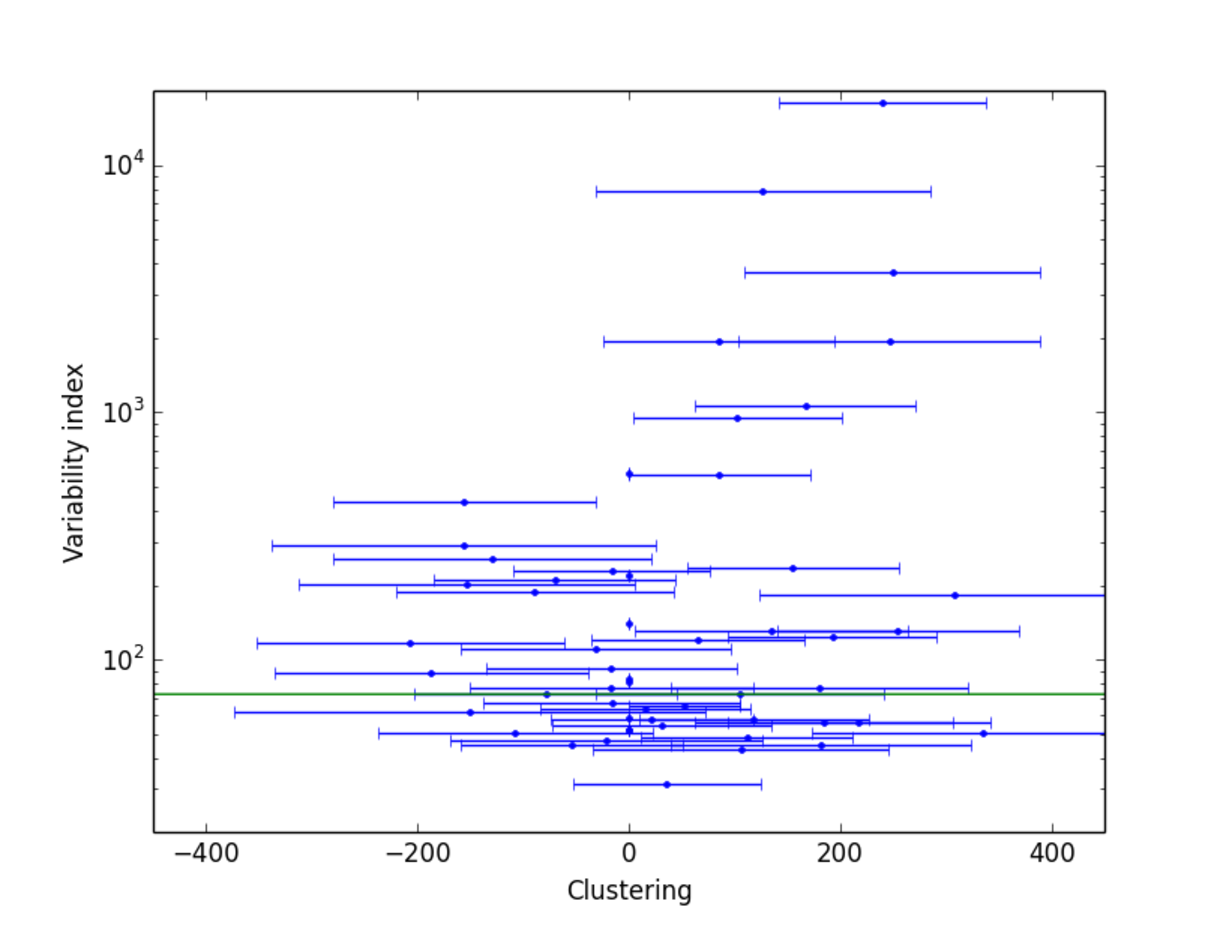
\includegraphics[width=3.5in]{figures/variability.pdf}
\caption{Variability \tsvar{} as a function of clustering amplitude \bgb{}. The horizontal green line shows the 99\% confidence limit for a variable source; all blazars above this line are considered variable at gamma-ray energies. 
\label{fig:variability}}
\end{figure}

%%%%%%%%%%%%
%%% CONCLUSIONS
%%%%%%%%%%%%

\section{Conclusions}\label{sec_conclusions}

We have computed the clustering amplitude for a sample of 757~blazars, the largest amount for which these have been determined by more than an order of magnitude. 

%%%%%%%%%%%%
%%% ACKNOWLEDGMENTS
%%%%%%%%%%%%

\acknowledgments
Funding for SDSS-III has been provided by the Alfred P. Sloan Foundation, the Participating Institutions, the National Science Foundation, and the U.S. Department of Energy Office of Science. The SDSS-III web site is http://www.sdss3.org/.

SDSS-III is managed by the Astrophysical Research Consortium for the Participating Institutions of the SDSS-III Collaboration including the University of Arizona, the Brazilian Participation Group, Brookhaven National Laboratory, University of Cambridge, Carnegie Mellon University, University of Florida, the French Participation Group, the German Participation Group, Harvard University, the Instituto de Astrofisica de Canarias, the Michigan State/Notre Dame/JINA Participation Group, Johns Hopkins University, Lawrence Berkeley National Laboratory, Max Planck Institute for Astrophysics, Max Planck Institute for Extraterrestrial Physics, New Mexico State University, New York University, Ohio State University, Pennsylvania State University, University of Portsmouth, Princeton University, the Spanish Participation Group, University of Tokyo, University of Utah, Vanderbilt University, University of Virginia, University of Washington, and Yale University.
\\

%\clearpage

%%%%%%%%%%%%
%%% BIBLIOGRAPHY
%%%%%%%%%%%%

\bibliography{blazar_refs,kwrefs}

\end{document}
